\documentclass[a4paper]{article}

\title{Low-Level Latent Space Skill Representations for Reuse in High-Level Environments}
\author{Andrew Fan}

\begin{document}
\maketitle
\section{Abstract}
While reinforcement learning (RL) algorithms have shown promising results in preforming robot locomotion tasks,
training times for large, complex environments take too long and are unfeasible. Many methods today require 
an agent to restart training for new environments, resulting in redudant skills being retrained every iteration.
Other methods require motion capture data for pretraining, which is unfeasible for robots that do not mimic living organisms.
In this paper, I propose a method for faster, completely unsupervised method for training on complex environments.

\section{Related Work}

\section{Reinforcement Learning Background}
\section{Autoencoders Background}
\section{Method}

\section{Results}
\begin{figure}
\centering
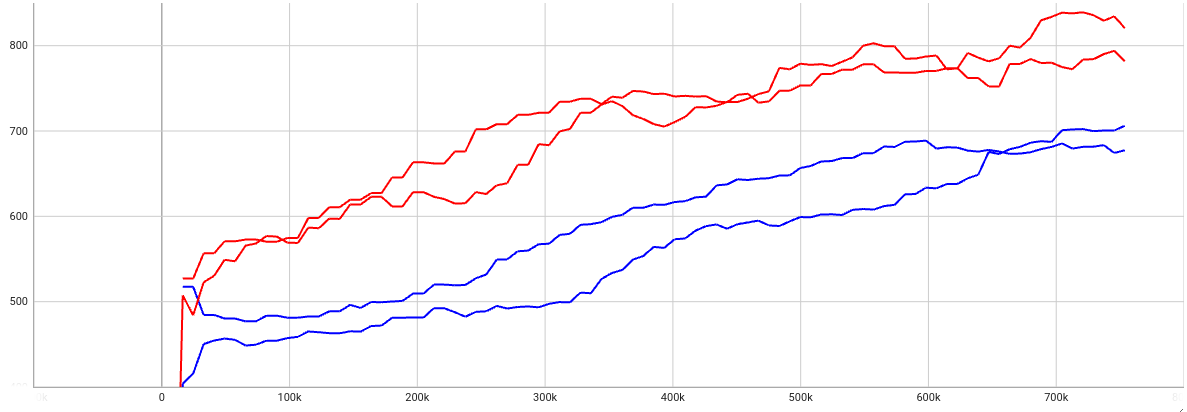
\includegraphics[width=0.25\linewidth]{./figs/obstacle-scratch-vs-autoencoder.png}
\caption{\label{fig:frog}This frog was uploaded via the file-tree menu.}
\end{figure}

\section{Future Work}
\end{document}
